\documentclass[10pt,a4paper]{article}
\usepackage{rpgcover} % Loads the original rpgmanual.sty and its fonts
\babelprovide[import]{ngerman}
\usepackage{xsavebox}
\RPGSetRunningTitle{Der Pfad der Schulden}
\hypersetup{pdftitle={Der Pfad der Schulden — Der letzte Wurf},pdfauthor={Jacopo Biscella}}
\RPGSetCoverWordSpace{.78em}
% Paragraph spacing and leading of the German adventure.
\setlength{\parskip}{3pt plus .5pt minus .5pt}
\linespread{1.06}\selectfont
% JPEG copies of the shared cover backgrounds (scripts/build-adventure-print-art.sh), as in the adventure.
\RPGSetFrontBackground{assets/engraved-front-background.jpg}\RPGSetBackBackground{assets/engraved-cover-background.jpg}
% The adventure's front-cover typography, with the overlay saved once (xsavebox) and reused on the
% contents page instead of being embedded twice.
\newcommand{\SentieroFrontCover}{%
 \clearpage\RPGCoverPagetrue\thispagestyle{empty}\null
 \xsavebox{SentieroOverlay}{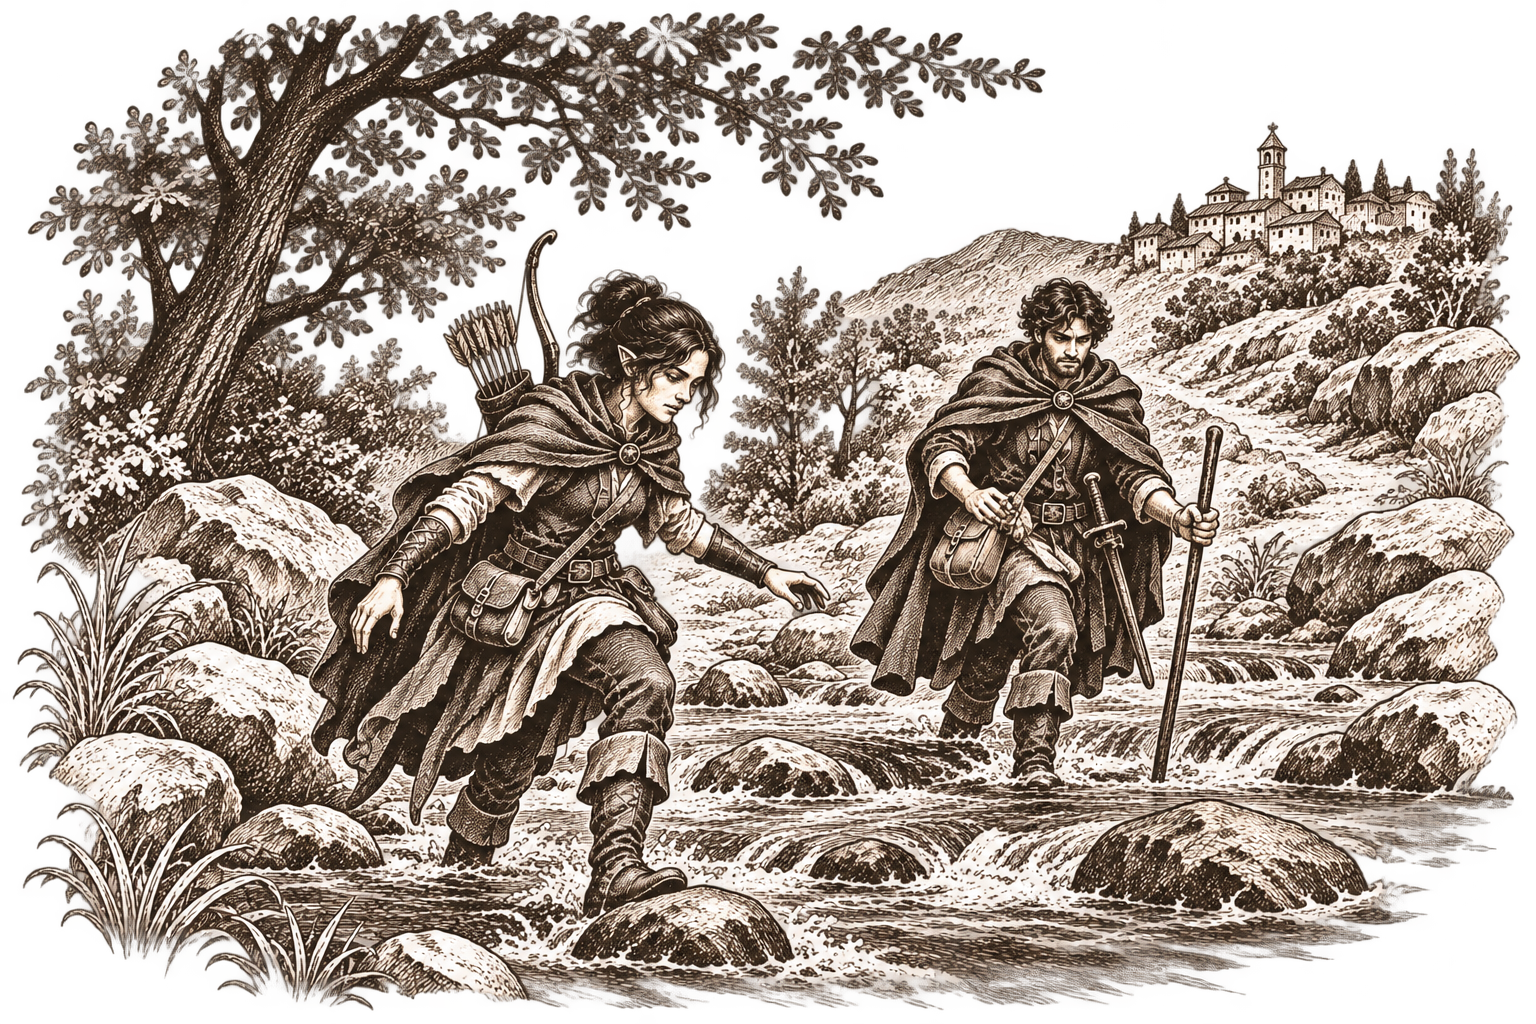
\includegraphics{assets/path-of-debts/front-overlay.png}}%
 \begin{tikzpicture}[remember picture,overlay,x=1mm,y=1mm]
  \RPGDrawBackground{\RPGFrontBackgroundFile}
  % Title and subtitle as on the adventure's cover: same sizes and positions in the cartouche.
  \node[align=center,text=coverink,text width=138mm,inner sep=0pt] at ($(current page.south west)+(105mm,248mm)$)
   {\RPGCoverTitleFont\fontsize{16.6}{20.7}\selectfont\spaceskip=\RPGCoverWordSpace\relax DER PFAD\\[1.0mm]DER SCHULDEN};
  \node[align=center,text=coverink,text width=135mm,inner sep=0pt] at ($(current page.south west)+(105mm,235mm)$)
   {\RPGCoverSubtitleFont\fontsize{9.0}{11.6}\selectfont Eine einführende Erzählung zu »Der letzte Wurf«};
  \node[inner sep=0pt,anchor=center] at ($(current page.south west)+(105mm,125mm)$)
   {\resizebox{150mm}{!}{\xusebox{SentieroOverlay}}};
  \node[align=center,text=coverink,text width=124mm,inner sep=0pt] at ($(current page.south west)+(105mm,25mm)$)
   {\RPGCoverTextFont\fontsize{12}{15}\selectfont Jacopo Biscella};
 \end{tikzpicture}
 \clearpage\RPGCoverPagefalse}
% Uses precisely the back background and the editable cover fonts from rpgcover.sty.
% This is text layout only: no substitute illustrations or background graphics.
\newcommand{\SentieroBackCover}{%
 \clearpage\pagenumbering{gobble}\RPGCoverPagetrue\thispagestyle{empty}\null
 \begin{tikzpicture}[remember picture,overlay,x=1mm,y=1mm]
   \RPGDrawBackground{\RPGBackBackgroundFile}
   \node[align=center,text=coverink,text width=170mm,inner sep=0pt]
     at ($(current page.south west)+(105mm,260mm)$)
     {{\RPGCoverTitleFont\fontsize{19}{23}\selectfont\spaceskip=\RPGCoverWordSpace\relax DER PFAD DER SCHULDEN}};
   \draw[coverink,line width=.45pt]
     ($(current page.south west)+(57mm,246mm)$)--($(current page.south west)+(153mm,246mm)$);
   % Blocks at the positions of the adventure's back cover: story at 240 mm, small-caps lines at
   % 197, second rule at 167, description at 162, closing line at 133.
   \node[anchor=north,align=left,text=coverink,text width=137mm,inner sep=0pt]
     at ($(current page.south west)+(105mm,240mm)$)
     {\RPGCoverTextFont\fontsize{10.4}{13.4}\selectfont
      Eine falsche Münze. Ein Brief ohne Empfänger. Zwei Reisende, die keinen Grund haben, einander zu trauen.\par\smallskip
      Nim Thistledown und Mara Veyne folgen der Königsstraße nach Hohlherd. Unterwegs lernen sie, dass ein Versprechen gefährlicher sein kann als eine Waffe und dass manche Entscheidungen Folgen haben, auch wenn niemand sie sieht.};
   \node[anchor=north,align=center,text=coverink,text width=140mm,inner sep=0pt]
     at ($(current page.south west)+(105mm,197mm)$)
     {\RPGCoverSubtitleFont\fontsize{13}{17}\selectfont
      Ein Prolog zu »Die Glocke von Hohlherd«};
   \draw[coverink,line width=.45pt]
     ($(current page.south west)+(57mm,167mm)$)--($(current page.south west)+(153mm,167mm)$);
   \node[anchor=north,align=left,text=coverink,text width=137mm,inner sep=0pt]
     at ($(current page.south west)+(105mm,162mm)$)
     {\RPGCoverTextFont\fontsize{10.4}{13.4}\selectfont
      Sieben Beispiele zeigen, wie am Tisch von Der letzte Wurf aus den Entscheidungen der Spieler Würfe, Dialoge und Folgen werden.};
   \node[anchor=north,align=center,text=coverink,text width=147mm,inner sep=0pt]
     at ($(current page.south west)+(105mm,133mm)$)
     {\RPGCoverSubtitleFont\fontsize{10.5}{13.2}\selectfont
      Die Geschichte endet, wo das Abenteuer beginnt.};
   \filldraw[fill=white,draw=coverink,line width=.55pt]
     ($(current page.south west)+(139mm,25mm)$) rectangle
     ($(current page.south west)+(187mm,55mm)$);
 \end{tikzpicture}
 \clearpage\RPGCoverPagefalse
}
% Dice icons for the "Am Tisch" boxes, drawn with TikZ (no font glyphs, so they work in every
% language). \Dado{n}: a kept d6 showing n; \Dado*{n}: a rolled die that is not kept (faded).
% \Su and \Giu: the rulebook's keep-highest and keep-lowest arrows, from FreeSerif.
% \Bersaglio: the TN to reach. \Riuscita and \Fallita: success and failure.
\newcommand\DadoPips[1]{%
  \ifcase#1\or \fill (.5,.5) circle (.1);
  \or \fill (.27,.73) circle (.1); \fill (.73,.27) circle (.1);
  \or \fill (.25,.75) circle (.09); \fill (.5,.5) circle (.09); \fill (.75,.25) circle (.09);
  \or \foreach \x/\y in {.27/.27,.27/.73,.73/.27,.73/.73}{\fill (\x,\y) circle (.095);}
  \or \foreach \x/\y in {.25/.25,.25/.75,.75/.25,.75/.75,.5/.5}{\fill (\x,\y) circle (.09);}
  \or \foreach \x/\y in {.28/.22,.28/.5,.28/.78,.72/.22,.72/.5,.72/.78}{\fill (\x,\y) circle (.085);}
  \fi}
\makeatletter
\newcommand\Dado{\@ifstar{\Dado@{.4}}{\Dado@{1}}}
\newcommand\Dado@[2]{\tikz[baseline=-.1em,x=.95em,y=.95em,opacity=#1]{%
  \draw[rpgbrown,line width=.5pt,rounded corners=1.2pt,fill=white] (0,-.12) rectangle (1,.88);
  \begin{scope}[shift={(0,-.12)},rpgink]\DadoPips{#2}\end{scope}}}
\makeatother
\newcommand\Su{{\fontspec{FreeSerif}↑}}
\newcommand\Giu{{\fontspec{FreeSerif}↓}}
\newcommand\Riuscita{\tikz[baseline=-.1em,x=1em,y=1em]{\draw[rpgbrown,line width=1.1pt,line cap=round,line join=round] (.08,.35)--(.38,.05)--(.92,.75);}}
\newcommand\Fallita{\tikz[baseline=-.1em,x=1em,y=1em]{\draw[rpgbrown,line width=1.1pt,line cap=round] (.15,.05)--(.85,.75) (.15,.75)--(.85,.05);}}
\newcommand\Bersaglio{\tikz[baseline=-.1em,x=1em,y=1em]{\draw[rpgbrown,line width=.6pt] (.5,.38) circle (.45) (.5,.38) circle (.25); \fill[rpgbrown] (.5,.38) circle (.08);}}
\begin{document}
% Select the language here: babel resets to its main language (english) at \begin{document}.
\selectlanguage{ngerman}
\RPGStartFrontMatter
\SentieroFrontCover
\RPGStartContents
\clearpage\thispagestyle{rpgfrontmatter}
\vspace*{9mm}
\begin{center}{\fontsize{27}{31}\selectfont\bfseries INHALT\par}\vspace{9pt}
{\color{rpgline}\rule{.76\linewidth}{.55pt}}\end{center}\vspace{8mm}
\begingroup
\makeatletter
\renewcommand{\l@section}[2]{\@dottedtocline{1}{0em}{4em}{\bfseries #1}{#2}}
\@starttoc{toc}
\makeatother
\endgroup
\vfill
\begin{center}\resizebox{.58\linewidth}{!}{\xusebox{SentieroOverlay}}\end{center}
\vfill
\begin{center}{\small\itshape Eine einführende Erzählung zu Der letzte Wurf\par}
\vspace{4pt}{\footnotesize Jacopo Biscella\par}\vspace{5pt}
{\footnotesize Diese Erzählung steht wie Der letzte Wurf unter der Lizenz Creative Commons Namensnennung–Weitergabe unter gleichen Bedingungen 4.0 International (CC BY-SA 4.0). Weitergabe und Bearbeitung, auch kommerziell, sind erlaubt, wenn der Autor genannt wird und abgeleitete Werke gleich lizenziert bleiben.\par}\end{center}
\clearpage
\RPGStartMainMatter
\RPGChapter{Eine schlechte Münze}
Die Münze hatte zwei Köpfe. Der eine trug die Krone des Königs, der andere das Gesicht eines Mannes, den der König vor zwanzig Jahren hatte hängen lassen.

Mara Veyne drehte sie zwischen Daumen und Zeigefinger. Das Kupfer war nur auf einer Seite abgegriffen. Wer sie geprägt hatte, wollte, dass der Schwindel nur kurz hielt: lange genug, um den Besitzer zu wechseln, nicht lange genug, um einem Steuereintreiber unter die Augen zu kommen.

»Ich hab dir doch gesagt, dass sie falsch ist«, sagte der Händler.

»Ich habe nichts anderes behauptet.«

»Warum starrst du sie dann seit einer halben Stunde an?«

»Um herauszufinden, wer sie benutzen will.«

Sie saßen an einem Tisch in der Poststation von Drei Furten. Seit vier Tagen regnete es. Die Königsstraße war zu einem langen Schlammstreifen geworden, auf dem Karren und Pferde nur mühsam vorankamen. Der Händler hatte Mara einen Platz auf dem Wagen für die Strecke nach Norden verkauft und dazu ein Versprechen: Er durfte das Warenbuch durchsehen, bevor sie die Kreuzung erreichten.

Dieses Versprechen, das hatte Mara begriffen, war mehr wert als die Fahrt.

Das Buch verzeichnete die Dörfer, die der Wagen belieferte. Darunter stand, in einer anderen Handschrift, \textbf{Hohlherd}. Neben den Namen hatte jemand ein rundes Zeichen gemalt und es dann durchgestrichen.

»Der Ort liegt nicht mehr auf meiner Strecke«, sagte der Händler, als er sah, wohin Mara blickte.

»Seit wann?«

»Seit der Holzpreis die Kosten der Fahrt nicht mehr deckt.«

»Und das Zeichen?«

Der Mann schlug das Buch zu. »Eine Kleinigkeit, um eine Lieferung im Blick zu behalten. Der Wagen fährt im Morgengrauen. Kommst du noch mit?«

Mara legte die Münze auf den Tisch, die Königsseite nach oben. »Ja.«

Er erzählte dem Händler nicht, dass er vor Jahren eine ähnliche Handschrift gesehen hatte, am Rand eines alten Registers. Er fragte auch nicht, warum jemand ein Datum weggekratzt und ein anderes hingeschrieben hatte. Er hatte gelernt, dass zu früh gestellte Fragen selbst die ungeschicktesten Lügner vorsichtig machen.

In jener Nacht schrieb er den Namen des Dorfes ans Ende seiner Notizen. Dann änderte er seine Route. Der Wagen würde nach Norden fahren. Mara würde an der Kreuzung den Waldpfad nehmen.
\begin{rpgnote}
\textbf{So liest man die Kästen.} In den Kästen \emph{Am Tisch} sind die Würfel abgebildet: \Dado{5}~behaltener Würfel, \Dado*{2}~beiseitegelegter Würfel, \Bersaglio~zu erreichender ZW, \Riuscita~Erfolg, \Fallita~Fehlschlag. Stufen wie auf dem Charakterbogen: Ungeübt 2W6\Giu\ (niedrigeren behalten), Kompetent 1W6, Experte 2W6\Su\ (höheren behalten), Herausragend 3W6\Su.
\end{rpgnote}
\begin{rpgexample}{Am Tisch · Der erste Wurf}
\textbf{Erzähler:} »Der Händler schlägt das Buch zu. Mara hat den Namen des Dorfes gesehen und ein weggekratztes Datum. Auf den ersten Blick ist das Datum unleserlich. Wie versuchst du, es zu entziffern?«

\textbf{Maras Spieler:} »Ich vergleiche die Reste der Ziffern mit den anderen Daten in derselben Handschrift. Ich nehme nicht Geschichte: Ich muss mich nicht erinnern, was passiert ist, ich muss getilgte Zeichen lesen.«

\textbf{Erzähler:} »Also Wissen, \Bersaglio\,ZW~4. Mara ist Experte: Würfle 2W6\Su, zwei Würfel, und behalte den höheren.«

\textbf{Maras Spieler:} »Ich würfle \Dado*{2}\,\Dado{5}: Ich behalte die 5.« \Riuscita

\textbf{Erzähler:} »Geschafft. Das Datum ist zwei Wochen alt, nicht von gestern. Den Namen des Dorfes kanntest du dagegen schon: Der hing nie vom Wurf ab.«

\emph{Gewürfelt wird, wenn der Ausgang ungewiss ist. Die Stufe Experte würfelt 2W6 und behält den besseren Würfel: Die 5 erreicht ZW~4. Ein unverzichtbarer Hinweis wird nie hinter einem Wurf versteckt.}

\end{rpgexample}
\RPGChapter{Der dritte Weg}
Nim Thistledown nahm den Beutel nicht sofort.

Der Fuhrmann hielt ihn geöffnet, mit der Miene eines Mannes, der Dank erwartet. Darin lagen sechs Silbermünzen und ein vierfach gefaltetes Blatt Papier.

»Die vereinbarte Bezahlung«, sagte er.

»Für den Weg, den wir beide kennen, vielleicht.«

»Für eine Lieferung.«

»Warum bringst du sie dann nicht selbst hin?«

Der Fuhrmann zeigte auf seinen Wagen, der mit gebrochenem Rad vor dem Stall stand. »Weil mir ein Pferd fehlt, ein Rad und die Lust, mich für einen Brief umbringen zu lassen.«

Nim faltete das Papier auf. Es war nicht versiegelt. Darauf standen zwei Zeilen: \emph{Die Hälfte der Schuld ist beglichen. Die andere Hälfte, in Nordsilber, wenn die Glocke verstummt.} Unten stand der Name einer Schenke in Hohlherd, aber nicht der Name dessen, für den der Brief bestimmt war.

»Wer hat dir das gegeben?«

»Ein Mann an der Kreuzung. Grauer Umhang, Kapuze auf. Er sagte die richtigen Worte, aber mit der Betonung an den falschen Stellen, wie jemand, der sie nach Gehör gelernt hat.«

Nim faltete das Blatt wieder zusammen. »Und sein Name?«

»Den hat er mir nicht genannt. Er hat mir Silber gegeben. Nimmst du's oder nicht?«

Nim nahm den Beutel, zählte die Münzen aber einzeln nach. Die sechste war dünn, fast glatt. »Es fehlen zwei.«

Der Fuhrmann seufzte und legte eine Münze dazu. Nim ging, bevor er es sich anders überlegen konnte.

Sie hatte nicht vor, den Brief blind abzuliefern. Es war genug Geld für drei Tage auf der Straße; zu viel für eine Nachricht ohne Namen. Und eine Glocke, die verstummen sollte, war kein Satz, den man unverstanden weitergab.

Der dritte Weg begann hinter den Ställen, wo der Schlamm nur wenige Fußspuren bewahrte. Ein schneller Pfad, laut Karte; ein verlassener, laut den Leuten aus der Gegend. Nim brach auf und zählte ihre Schritte bis zur ersten Gabelung.
\RPGChapter{Der umgestürzte Baum}
Mara traf Nim nach Mittag, vor einem Stamm, der den Pfad versperrte.

Nim untersuchte den Boden. Sie hatte die Tasche auf einen Stein gestellt und einen Zweig zwischen den Zähnen.

»Ist der Wald gesperrt?«, fragte Mara.

»Kommt drauf an, wie sehr du Abkürzungen magst.«

»Nicht sehr.«

»Dann haben wir etwas gemeinsam.«

Der Stamm einer Buche lag quer über dem Weg, die Wurzeln noch in der Erde. Er war vor Kurzem umgestürzt. Die Blätter waren grün, die Rinde feucht. Es hatte keinen Wind gegeben, der stark genug gewesen wäre, ihn zu fällen.

Mara hockte sich hin, um einen Splitter zu betrachten. Aus dem Schnitt sickerte klarer Saft.

»Eine Axt«, sagte er.

»Zwei«, erwiderte Nim. »Einer hat auf dieser Seite gearbeitet, ein anderer auf der anderen.«

Mara betrachtete die Kerben: parallel, regelmäßig, zu tief unten für jemanden, der Brennholz wollte. »Sie haben ihn nur gefällt, um den Pfad zu sperren.«

»Es gibt Spuren, die zurückführen. Auf der anderen Seite keine.«

»Du kannst Spuren lesen?«

»Ich sehe, wo jemand versucht hat, sie zu verwischen.«

Mara lächelte leicht. Nim schlüpfte unter dem Stamm hindurch, kam mit schlammigem Ärmel wieder hervor und zeigte auf eine schmale Lücke zwischen den Wurzeln. »Man kommt durch, aber wer einen Wagen hat, muss umkehren.«

»Und wer Bücher hat?«

»Kommt drauf an, wie viele.«

Mara klopfte auf seine Umhängetasche. »Zu viele.«

Ihre Namen tauschten sie erst aus, als sie das Hindernis hinter sich hatten. Ein großer Vertrauensbeweis war das nicht. Aber Mara hörte auf, jedes Mal die Hand an den Verschluss seiner Tasche zu legen, wenn Nim näher kam.
\RPGChapter{Der Erdrutsch}
Den Erdrutsch fanden sie fast eine Stunde später.

Der Pfad verlief am Hang entlang, über einem angeschwollenen Bach. Auf etwa zwanzig Schritten war er verschwunden: Der Regen hatte einen Streifen des Hangs abgerissen, und an seiner Stelle zog sich eine Zunge aus Schlamm und Steinen bis hinunter zum Wasser. Hin und wieder löste sich ein Stein und rollte ohne Eile hinab. Jemand war am Vortag hier entlanggegangen: Die Spuren reichten bis zur Mitte und verschwanden unter einem jüngeren Abgang.

Nim musterte den Hang. »Wir könnten zur Furt zurückgehen.«

»Wie lange würde das dauern?«

»Zwei Stunden, vielleicht drei.«

Mara blickte auf. Die Wolken schoben sich wieder vor die Sonne. »Und wie weit ist es bis zum Dorf?«

»Noch ein halber Tag.«

»Dann kämen wir im Dunkeln an.«

Nim betrachtete den Erdrutsch. Wo der Schlamm den Fels freigelegt hatte, fand ein Fuß Halt; anderswo gab die Erde bei der leisesten Berührung nach. »Wenn ich schnell und leicht hinübergehe, hat der Hang keine Zeit zu rutschen.«

»Du könntest auch stürzen.«

»Das ist eine der Möglichkeiten.«

Mara zog den Riemen seiner Tasche vor der Brust fest. »Dann gehst du nicht allein. Ich gehe hinter dir, setze die Füße dorthin, wo du deine hinsetzt, und halte dich am Gürtel. Wenn du rutschst, halte ich dich.«

»Und wenn du rutschst, ziehst du mich mit runter.«

»Dann sorg dafür, dass ich nicht rutsche.«

Nim sah ihn einen Moment lang an. Dann wandte sie sich dem Erdrutsch zu und ging los. Mara folgte, eine Hand fest an ihrem Gürtel.

Auf halbem Weg gab unter Nims Fuß eine Scholle nach. Der Schlamm bewegte sich auf einmal, wie eine Decke, die man von einer Seite wegzieht. Nim kippte nach vorn; Mara stemmte die Fersen gegen einen Stein und zog. Der Gürtel hielt. Einen Augenblick standen sie still, während die gelösten Steine zum Bach hinunterrollten.

Dann fand Nim Fels, und Mara folgte ihr Schritt für Schritt.

Als sie die andere Seite erreichten, zitterten Mara die Beine. Nim drehte sich um: Der Übergang war schon unter einer frischen Schlammschicht verschwunden.

»Zwei Stunden gespart«, sagte sie.

»Die zehn Lebensjahre, die ich gerade verloren habe, hast du nicht mitgerechnet.«

»Die standen nicht auf der Karte.«
\begin{rpgexample}{Am Tisch · Hinüberkommen und helfen}
\textbf{Erzähler:} »Der Erdrutsch ist noch in Bewegung. Ihn zu überqueren ist Geschick, \Bersaglio\,ZW~4. Bei einem Fehlschlag rutschst du auf den Bach zu.«

\textbf{Nims Spielerin:} »Nim ist Expertin in Geschick: 2W6\Su. Kann Mara mir helfen?«

\textbf{Maras Spieler:} »Ich gehe direkt hinter ihr und halte sie am Gürtel. Wenn sie rutscht, halte ich sie.«

\textbf{Erzähler:} »Ihr geht gemeinsam hinüber, und es würfelt, wer vorangeht: Nim. Mara ist in Geschick Ungeübt und hat keine Fertigkeit, die hilft: Bei derselben Probe würde er nicht auf Stufe Experte würfeln, also ist seine Hilfe inkompetente Hilfe. Sie gibt Nims Wurf einen Würfel dazu, aber der ZW steigt von 4 auf 5: Zwei Leute auf dem Schlamm lösen mehr Steine. Nehmt ihr an?«

\textbf{Nims Spielerin:} »Ja. Wenn ich allein ausrutsche, habe ich nichts, woran ich mich festhalten kann.«

\textbf{Erzähler:} »Dann würfelt Nim 3W6\Su\ gegen \Bersaglio\,ZW~5.«

\textbf{Nims Spielerin:} »Ich würfle \Dado*{1}\,\Dado*{4}\,\Dado{5}: Ich behalte die 5.« \Riuscita

\textbf{Erzähler:} »Ihr seid drüben. Auf halbem Weg gibt unter Nim eine Scholle nach, und Mara hält sie am Gürtel. Auf der anderen Seite dreht ihr euch um: Der Übergang ist schon unter dem Schlamm verschwunden. Hier kommt kein Wagen mehr durch.«

\emph{Inkompetente Hilfe gibt +1W6, erhöht aber den ZW um 1. Mit 1, 4 und 5 erreicht Nim den neuen ZW~5. Maras Hand am Gürtel ist die Art, wie die Hilfe in die Geschichte eingeht: Sie ersetzt den Wurf nicht.}

\end{rpgexample}
\RPGChapter{Zwei Leute auf der Straße}
Sie gingen, bis der Pfad so breit wie eine Straße wurde. Dann sahen sie den Wagen.

Er hatte hohe Räder, eine mit Wachstuch bedeckte Ladefläche und ein graues Pferd, das die untersten Blätter eines Haselstrauchs fraß. Der Kutscher schlief auf dem Bock, den Hut über dem Gesicht. Eine Frau beugte sich über die Nabe des rechten Rads.

»Können wir helfen?«, fragte Mara.

Die Frau richtete sich auf. Ihre Hände waren schwarz vor Schmiere, und am Gürtel hing ein Arbeitsmesser. »Wenn ihr einen Ersatzbolzen habt.«

Nim sah sich das Rad an. »Du musst ihn nicht austauschen. Die Klammer ist verbogen.«

»Und woher willst du das wissen?«

»Weil der Bolzen noch an seinem Platz sitzt.«

Die Frau reichte ihr wortlos den Hammer. Nim hockte sich hin, hebelte mit einem flachen Stein und setzte drei genaue Schläge. Die Klammer war wieder fast gerade.

»Versuch es jetzt«, sagte sie.

Die Frau zog am Rad. Es drehte sich.

Der Kutscher wachte von dem Lärm auf. Er fragte, wer sie seien, warum sie den Wagen anfassten und ob sie ihn ausrauben wollten. Die Frau sagte ihm, er solle still sein.

»Fahrt ihr nach Hohlherd?«, fragte Mara.

Die Frau hörte auf, sich die Hände abzuwischen. »Bis vor Kurzem sind wir dort durchgekommen.«

»Und jetzt?«

»Jetzt verlieren wir lieber einen Tag.«

Mehr wollte sie nicht sagen, aber sie gab ihnen ein Stück Brot und einen harten Käse, in ein Blatt gewickelt. Als der Kutscher abgelenkt war, sprach sie leise.

»Die Straße nach Norden ist voller Männer, die Wegzoll verlangen, ohne ein Recht darauf zu haben. Sie tragen keine Uniform. Einer von ihnen hat früher eine getragen.«

»Wo?«, fragte Nim.

»An der Kreuzung der drei Steine. Wenn ihr ihm begegnet, sagt nicht, dass ihr mir geholfen habt.«

Mara drängte sie nicht. Bevor sie weitergingen, kauerte Nim an den Radspuren. Zwischen den Hufabdrücken waren andere, von zwei Fußgängern: Sie waren dem Wagen fast bis zum Haselstrauch gefolgt und dann nach Norden umgekehrt.

»Das ist keine Warnung vom Hörensagen«, sagte Nim zu der Frau. »Ihr seid ihnen schon begegnet.«

Die Frau betrachtete die Spuren und nickte. »Einer ist jung. Der andere zeigt sich nur, wenn er muss.«

Sie ließ sie mit einem Nicken ziehen und ging zurück zum Wagen.
\begin{rpgexample}{Am Tisch · Wenn eine Fertigkeit den Wurf verändert}
\textbf{Erzähler:} »Die Klammer ist verbogen. Nim, wie versuchst du, sie zu richten?«

\textbf{Nims Spielerin:} »Mit dem Hammer der Fuhrfrau und einem Stein als Widerlager.«

\textbf{Erzähler:} »Eine richtige Reparatur wäre Wissen mit Handwerk. Hier musst du die Klammer aber nur mit drei genauen Schlägen geradebiegen: Geschick, \Bersaglio\,ZW~4. Bei einem Fehlschlag kannst du sie abbrechen.«

\textbf{Nims Spielerin:} »Nim ist Expertin in Geschick: 2W6\Su. Keine ihrer Fertigkeiten hat mit Hämmern zu tun, also keine zusätzliche Stufe. Ich würfle \Dado*{3}\,\Dado{5}: Ich behalte die 5.« \Riuscita

\textbf{Erzähler:} »Das Rad dreht sich wieder. Als ihr aufbrecht, bemerkst du Fußspuren neben den Radspuren. Willst du sie untersuchen?«

\textbf{Nims Spielerin:} »Ja. Nim hat Überleben, eine Fertigkeit des Geschicks, die genau fürs Spurenlesen da ist.«

\textbf{Erzähler:} »Herauszufinden, wer dem Wagen gefolgt ist, ist \Bersaglio\,ZW~4. Geschick Experte plus Überleben: Du steigst eine Stufe auf, zu Herausragend. Würfle 3W6\Su.«

\textbf{Nims Spielerin:} »Ich würfle \Dado*{2}\,\Dado*{4}\,\Dado{6}: Ich behalte die 6.« \Riuscita

\textbf{Erzähler:} »Du erkennst zwei Spurenfolgen: Sie sind dem Wagen gefolgt und dann nach Norden abgebogen. Die Frau bestätigt, dass sie den falschen Zöllnern schon begegnet ist.«

\emph{Die Werte sind die auf Nims Charakterbogen: Expertin in Geschick, mit Überleben und ohne Handwerk, das ohnehin eine Fertigkeit des Wissens ist. Eine passende Fertigkeit verbessert den Wurf um eine Stufe. Eine einzelne 6 ist kein kritischer Erfolg: Dafür braucht es mindestens zwei.}

\end{rpgexample}
\RPGChapter{Die Kreuzung der drei Steine}
An der Kreuzung gab es drei Wegsteine, doch nur zwei standen noch. Der dritte lag auf der Seite, halb im Gras verborgen. Jemand hatte ein frisches Zeichen ins Moos geritzt: einen Kreis, durch den eine Linie lief.

Nim erkannte darin das Zeichen eines fahrenden Steuereintreibers. Sie hatte es auf echten und gefälschten Quittungen gesehen, öfter auf gefälschten als auf echten.

»Der Wegzoll ist ein Schwindel«, sagte sie.

»Das ist keine Überraschung.«

»Die Wahl des Ortes schon. Hier gibt es nichts, was sich zu schützen lohnt.«

»Eine Straße«, erwiderte Mara, »ist auch dann nützlich, wenn nichts um sie herum ist.«

Es folgte ein kurzes Schweigen. Dann kam eine Stimme hinter den Büschen hervor.

»Zwanzig Münzen fürs Durchkommen.«

Der Mann, der ins Freie trat, war jung. Er trug einen zu großen Mantel, einen Speer mit rostiger Spitze und zwei ungleiche Stiefel. Ein zweiter Mann blieb zwischen den Bäumen, wo der Pfad wieder enger wurde.

»Zwanzig?«, wiederholte Nim. »Der König muss ja großzügig zu seinen Eintreibern geworden sein.«

»Ich habe nicht gesagt, dass ich zum König gehöre.«

»Stimmt. Der König hätte wenigstens so viel Verstand gehabt, jemanden mit einer Quittung zu schicken.«

Der junge Mann senkte den Speer auf Nims Brust. Mara trat einen Schritt vor.

»Warte«, sagte er zu dem jungen Mann. »Wer hat dir befohlen, hier zu stehen?«

»Zahl oder kehr um.«

»Wenn du uns durchlässt«, fuhr Mara fort, »bekommst du keinen Ärger. Wenn dich jemand zum Kassieren geschickt hat, hat er dir auch gesagt, wohin du das Geld bringen sollst.«

Der junge Mann zögerte. Der Versteckte hustete.

Nim fuhr herum und blickte an ihnen vorbei. »Da ist jemand auf der Straße.«

Der junge Zöllner folgte einen Augenblick lang ihrem Blick. Das genügte. Nim drückte die Speerspitze nach unten und ging an ihm vorbei. Mara folgte ihr, ohne zu rennen.

Zwischen den Bäumen fluchte jemand. Niemand folgte ihnen.

Sie gingen hundert Schritte schweigend, dann sagte Mara: »Hinter uns war niemand.«

»Das habe ich auch nicht behauptet.«

»Du hast gesagt, da ist jemand auf der Straße.«

»Nein. Ich habe gesagt: ›Da ist jemand auf der Straße.‹ Wir waren auf der Straße.«

Mara schüttelte den Kopf. Er lachte nicht, aber man sah ihm an, dass er es gern getan hätte.
\begin{rpgnote}[fontupper=\normalfont]\textbf{Junger Zöllner} \emph{ZW S3/G3 · Kompetent · 2 Wunden · Speer (2Wu) · keine Rüstung.} \emph{Verhalten: »Befolgt Befehle, will aber niemanden töten.«}\end{rpgnote}
\begin{rpgexample}{Am Tisch · Ein Vergleichswurf}
\textbf{Erzähler:} »Der junge Mann mit dem Speer versperrt euch den Weg. Der andere wartet zwischen den Bäumen. Was tut ihr?«

\textbf{Nims Spielerin:} »Ich tue so, als sähe ich jemanden hinter ihnen, um sie abzulenken.«

\textbf{Erzähler:} »Der junge Mann beäugt dich misstrauisch: Das ist ein Vergleichswurf auf Wissen, und es gibt keinen ZW, den du erreichen musst. Nim ist in Wissen Ungeübt und hat keine Täuschung: Würfle 2W6\Giu\ und behalte den niedrigeren. Der junge Mann ist Kompetent: 1W6.«

\textbf{Nims Spielerin:} »Ich würfle \Dado{5}\,\Dado*{6}: Ich behalte die 5.«

\textbf{Erzähler:} »Der junge Mann würfelt \Dado{2}. Deine 5 ist höher: Er dreht sich um und senkt einen Moment lang den Speer. Ihr könnt an ihm vorbei, während Mara ihn mit Reden beschäftigt.« \Riuscita

\textbf{Maras Spieler:} »Ich sage ihm, er soll uns gehen lassen: Ich will ihm nicht wehtun.«

\emph{Bei einem Vergleichswurf würfeln beide Seiten, und das höhere Ergebnis gewinnt; Gleichstand bedeutet eine Pattsituation. Es gibt keinen festen ZW. Der Wurf eröffnet eine Gelegenheit; er entscheidet nicht allein über alles, was danach geschieht.}

\end{rpgexample}
\RPGChapter{Die Scheune}
Kurz vor Sonnenuntergang regnete es wieder. Die beiden Reisenden fanden Unterschlupf in einer verlassenen Scheune, zweihundert Schritte von der Straße entfernt. Eine Wand war eingestürzt; das Dach aber hielt.

Nim raffte einen Armvoll trockenes Stroh zusammen und schob es an die Wand. Mara legte seine Bücher auf eine leere Kiste. Aus dem hinteren Teil der Scheune kam ein Geruch nach nasser Wolle.

Sie waren nicht allein.

Hinter der Futterkrippe saß ein Mädchen, in eine Decke gewickelt, die ihr zu groß war. Das Haar klebte ihr an der Stirn, und sie hielt einen Mehlsack umklammert. Neben ihr schlief ein magerer Hund.

»Wir wollen deinen Sack nicht«, sagte Mara.

»Er gehört nicht mir.«

»Wem gehört er?«

Das Mädchen schwieg. Nim setzte sich auf die andere Seite der Scheune und begann, ihr Messer mit einem Lappen zu säubern. Sie tat es so, dass die Klinge nie auf das Mädchen zeigte.

»Hast du einen Namen?«, fragte Mara.

»Tessa.«

»Wohin gehst du, Tessa?«

»Zu meinem Onkel.«

»Wo wohnt er?«

»Weiter vorn.«

Mehr mussten sie nicht wissen, um zu sehen, dass sie Angst hatte. Mara packte das Brot aus, das ihnen die Fuhrfrau gegeben hatte, und brach ein Stück ab. Er legte es auf die Kiste zwischen ihnen.

Tessa wartete, bis Mara zu seiner Decke zurückgekehrt war, dann nahm sie das Brot.

Später, als der Hund aufwachte, erzählte das Mädchen von Männern, die nachts zu ihr nach Hause gekommen waren, auf der anderen Seite des Tals, um das Korn zu holen. Ihre Mutter hatte sie mit dem letzten Sack Mehl zum Onkel geschickt. Auf halbem Weg hatte der Regen sie überrascht.

»Morgen früh können wir dich bis zur nächsten Gabelung begleiten«, sagte Mara.

Nim sagte nichts. Am nächsten Morgen war sie aber die Erste, die aufstand.
\begin{rpgexample}{Am Tisch · Merkmal und Bürde}
\textbf{Erzähler:} »Das Mädchen will nicht reden und hält den Sack fest. Was tut ihr?«

\textbf{Maras Spieler:} »Ich gebe ihr etwas zu essen und lasse ihr Zeit. Ich will sie nicht ausfragen.«

\textbf{Erzähler:} »Dafür braucht es keinen Wurf: Brot kauft dir nicht ihr Vertrauen, aber es zeigt ihr, dass ihr keine unmittelbare Bedrohung seid. Mara, gibt es in deinem Merkmal oder deiner Bürde etwas, das diese Entscheidung für ihn wichtig macht?«

\textbf{Maras Spieler:} »Ja. Maras Bürde ist ein Versprechen, das er nicht halten kann. Tessa soll ihn daran erinnern.«

\textbf{Erzähler:} »Dann verlange ich nicht, dass du jetzt alles erzählst. Heute Nacht bleibt Mara länger wach als nötig, um sicherzugehen, dass Tessa in Sicherheit ist.«

\textbf{Nims Spielerin:} »Ich könnte das Mädchen fragen, wer bei ihr eingebrochen ist, aber ich tue es nicht. Sie soll uns wenigstens so weit vertrauen, dass sie isst.«

\textbf{Erzähler:} »Diese Entscheidung hat ihren Preis: Heute Nacht erfahrt ihr nicht, wer das Korn genommen hat. Dafür zeigt Tessa euch am Morgen den kürzesten Weg zu ihrem Onkel.«

\textbf{Maras Spieler:} »Wir hätten sie also ausfragen können, aber dann wäre die Szene anders verlaufen?«

\textbf{Erzähler:} »Ja. Das Spiel verlangt nicht, dass jede Frage sofort beantwortet wird. Ihr habt euch entschieden, Tessa zu schützen, und jetzt folgt die Reise dieser Entscheidung.«

\emph{Merkmale und Bürden lenken Entscheidungen und eröffnen erzählerische Zwickmühlen; für sich allein geben sie keine Zahlenboni. Ihre Wirkung entsteht aus der Situation und aus den Entscheidungen der Spieler.}

\end{rpgexample}
\RPGChapter{Die Schlucht}
Hinter der Scheune stieg der Pfad zwischen zwei Felswänden an. Auf halber Höhe ragte ein Felsbrocken über den Weg. Dünne Wurzeln waren in ihn hineingewachsen, und eine davon hielt eine lose Steinplatte zusammen.

Nim bemerkte es, weil ein Krümel Erde neben ihrem Stiefel fiel. Sie blickte auf und sah die Lücke unter dem Stein.

»Halt.«

Tessa blieb sofort stehen. Mara machte noch einen halben Schritt.

Von weiter oben kam ein dumpfer Schlag, dann ein zweiter. Eine Wildziege lief den Grat entlang. Die Steine, die sie lostrat, waren nicht groß, aber sie reichten, um die Platte zu erschüttern.

»Zurück«, sagte Nim.

Das Mädchen drückte sich an die Felswand. Mara packte sie am Handgelenk und zog sie unter einen kleinen Überhang. Nim blieb einen Augenblick zu lange ungeschützt.

Die Platte gab nach. Sie fiel nicht in einem Stück: Sie zerbrach an einem Felsvorsprung und übersäte den Pfad mit Bruchstücken. Nim wich den größten Stücken aus und bekam einen Stein an die Schulter. Der Schlag zwang sie in die Knie.

Als der Lärm verstummte, lief Mara zu ihr.

»Kannst du den Arm bewegen?«

Nim versuchte es. »Ja.«

»Tut es weh?«

»Wenn nicht, würde ich mir Sorgen machen.«

Tessa kam aus dem Unterschlupf hervor, blass, aber unverletzt. Nim bedeutete ihr, vorauszugehen.

Für den Rest des Aufstiegs sagte sie wenig. An jeder Biegung vergewisserte sie sich, dass das Mädchen noch vor ihr war. Mara beobachtete sie, ohne es sich anmerken zu lassen. An der nächsten Biegung packte er, ohne zu fragen, die schwerste Last aus Nims Tasche in seine eigene.
\begin{rpgexample}{Am Tisch · Ein Fehlschlag verändert die Szene}
\textbf{Erzähler:} »Die Platte löst sich. Nim steht ungeschützt: Geschick, \Bersaglio\,ZW~5. Bei einem Fehlschlag treffen dich die Trümmer.«

\textbf{Nims Spielerin:} »Nim ist Expertin: 2W6\Su. Ich würfle \Dado*{2}\,\Dado{3}. Ich behalte die 3: Fehlschlag.« \Fallita

\textbf{Erzähler:} »Ein Stein trifft dich an der Schulter. Du kannst noch gehen, aber der Schmerz zählt als Zustand: Bei Handlungen, für die du diesen Arm brauchst, hast du −1 Stufe, bis die Schulter behandelt wird oder verheilt. Tessa ist in Sicherheit, dank des Unterschlupfs, den Mara gefunden hat.«

\textbf{Nims Spielerin:} »Dann lasse ich Mara die schwere Tasche tragen.«

\emph{Ein Fehlschlag erzeugt eine genaue, begrenzte Folge, und die Geschichte geht weiter. Ein Zustand nimmt den Würfen, bei denen er zählt, eine Stufe, bis er behoben ist. Er ist keine Wunde und kostet keine Lebenspunkte.}

\end{rpgexample}
\RPGChapter{Drei Teller auf dem Tisch}
Kurz vor Mittag erreichten sie den Hof von Tessas Onkel. Auf dem Küchentisch standen drei Keramikteller, zum Trocknen ans Fenster gestellt. Das Haus war leer, aber das Kaminfeuer war erst am Morgen angezündet worden.

Mara klopfte. Keine Antwort.

Nim ging um das Gebäude herum. Hinter dem Stall fand sie einen Mann, der Holz hackte, ein Knie verbunden, das Hemd am Hals offen.

»Wenn ihr Essen sucht, ich hab keins«, sagte der Mann.

»Wir suchen sie«, erwiderte Nim und zeigte auf Tessa.

Der Mann ließ die Axt fallen. Einen Moment lang rührte er sich nicht. Dann überquerte er den Hof so schnell, dass Tessa kaum Zeit hatte, die Arme zu heben, bevor er sie an seine Brust drückte.

Mara wandte sich der Straße zu. Es schien ihm angebracht, die beiden einen Moment für sich zu lassen.

Der Onkel bot Suppe an, einen Platz am Feuer und eine Nacht unter seinem Dach. Nim nahm die Suppe an und lehnte den Rest ab. Mara wollte Hohlherd vor Einbruch der Dunkelheit erreichen.

Tessa drückte Nim einen Knochenknopf in die Hand, den einzigen, den sie vom Mantel ihres Vaters behalten hatte. »Für die Schlucht«, sagte sie.

Nim wollte ihn ihr zurückgeben. Das Mädchen schloss Nims Finger um den Knopf und lief zu ihrem Onkel.

»Das ist eine schlechte Idee«, sagte der Mann.

»Das hören wir in letzter Zeit öfter«, erwiderte Mara.

»Dann solltet ihr vielleicht zuhören.«

»Was geht dort unten vor?«

Der Onkel sah zu Tessa, die jetzt am Tisch aß. »Ich weiß nicht genug, um es euch zu sagen. Die Letzten, die aus dem Dorf kamen, wollten nicht reden. Und wer von dort kommt, bleibt nicht mehr stehen, um zu reden.«

»Nicht einmal ein Name?«

»Ich habe den alten Bram erwähnen hören. Aber ich weiß nicht, was aus ihm geworden ist.«

Mara dachte an den Brief in Nims Tasche, den er am Vorabend erspäht hatte. Den Inhalt kannte er noch nicht.
\RPGChapter{Der Brief und die Schuld}
Nach dem Mittagessen brachen sie wieder auf. Von dort führte die Straße hinab zum Wald. Nim sprach als Erste.

»Ich wurde dafür bezahlt, einen Brief in die Schenke von Hohlherd zu bringen.«

Mara streckte die Hand aus. »Darf ich ihn lesen?«

\emph{Die Hälfte der Schuld ist beglichen. Die andere Hälfte, in Nordsilber, wenn die Glocke verstummt.}

»Da steht kein Name«, sagte Mara.

»Da steht eine Schenke. Und es gab einen Mann an der Kreuzung, der gut bezahlt hat.«

»Zu gut.«

Mara las die letzte Zeile erneut. In den Registern, die er studiert hatte, stand Hohlherd immer zusammen mit seiner Glocke.

Nim hielt das Blatt gegen das Licht. Am Rand waren zwei Nadellöcher, dicht beieinander. Mara nahm die falsche Münze, die er aufbewahrt hatte, aus seinem Notizbuch. Zu Beginn der Reise war sie ihm wie eine Kuriosität vorgekommen. Jetzt erkannte er den Stempel im Wachs zwischen den beiden Löchern wieder: zwei voneinander abgewandte Köpfe, einer gekrönt, einer barhäuptig.

»Dieses Papier ist durch die Hände dessen gegangen, der diese Münzen prägt.«

Nim dachte an die Zöllner an der Kreuzung. »Ein Schwindel mit einer Nachricht obendrein?«

»Vielleicht. Oder jemand kauft Schweigen. So oder so steht nicht da, wer ihn bekommen soll.«

Hinter ihnen knackte ein Ast.

Der junge Mann mit dem Speer war zurückgekommen. Diesmal war der Mann bei ihm, der sich zwischen den Bäumen versteckt gehalten hatte: älter, eine Narbe am Kiefer, ein Lederwams und ein Kurzschwert an der Seite. Sie blieben auf dem Pfad stehen, ein Dutzend Schritte entfernt.

»Die Lieferung ist abgesagt«, sagte der Ältere. »Gebt das Papier zurück und behaltet das Silber.«

»Welches Papier?«, fragte Nim.

Der Mann ließ einen Beutel vor ihre Füße fallen. Das Klirren des Silbers war deutlich zu hören. »Ihr könnt zweimal dafür bezahlt werden, keine Fragen zu stellen.«

Mara sah den jungen Mann an, der den Blick auf seine Stiefel gesenkt hielt. »Du hast gesagt, ihr kassiert Wegzoll. Jetzt sammelt ihr die Post ein?«

»Letztes Angebot«, antwortete der andere. Er legte die Hand an den Griff.

Nim trat zur Seite. Nicht auf den Beutel zu: auf einen Stamm zu, an dem jeder nur einzeln vorbeikam. Mara verstand und stellte sich hinter sie. Im Schlamm packte der junge Mann den Speerschaft fester, ohne ihn zu heben.

Nim spürte Tessas Knochenknopf in der Tasche. Der Beutel im Schlamm hätte eine ganze Reisesaison bezahlt; ein Stück weiter zurück hatten beide etwas gewagt für ein Mädchen, das nichts besaß.

»Willst du für dieses Papier kämpfen?«, fragte Mara, so leise, dass die Männer es nicht hörten.

»Nein«, sagte Nim. »Ich will es nicht verkaufen.«

Der Mann mit der Narbe zog sein Schwert. Nim warf ihm ihren Umhang über den Schwertarm und stieß ihn gegen den Stamm. Der junge Mann trat vor, doch Mara hielt ihn mit erhobener, offener Hand auf.

»Du hast schon einen Ausweg«, sagte er zu ihm. »Nutz ihn nicht, um zuzuschlagen.«

Der junge Mann zögerte. Der Mann mit der Narbe befreite seinen Arm und holte aus: Die Klinge glitt unter dem Umhang durch und schnitt Nim in die Seite. Nim wich bis zum Stamm zurück. Der Mann hätte ihr nachsetzen können. Stattdessen sah er den Gefährten an, der reglos mit gesenktem Speer stand, und spuckte in den Schlamm.

»Behaltet das Papier. Die Bezahlung holt ihr euch bei den Toten ab.«

Nim und Mara gingen davon, ohne den zweiten Beutel aufzuheben. Sie warteten, bis sie über der Anhöhe waren, ehe sie stehen blieben.

Mara war außer Atem. »Du hättest dich nicht für einen Brief in Gefahr bringen sollen.«

Nim betastete ihre Seite. Der Schnitt blutete, aber sie konnte noch gehen. »Ich hab's nicht für den Brief getan.«

»Wofür dann?«

»Um nicht die Sorte Mensch zu sein, die man so leicht kaufen kann.«

Die Antwort überraschte Mara mehr als das Schwert. Nim nahm den Brief, faltete ihn und gab ihn Mara.

»Du erkennst geschriebene Lügen besser als ich. Behalte ihn, bis wir jemanden finden, dem wir ihn zeigen können.«

Mara steckte den Brief neben die falsche Münze. Ihre Abmachung war einfach: Sie würden ihn keinem Fremden aushändigen, nur weil jemand sie bezahlt hatte. Sie würden von demjenigen eine Erklärung verlangen, der für das Dorf verantwortlich war. Nim verzichtete auf den Lohn, der ihr für die Lieferung versprochen war; Mara, der es immer vorgezogen hatte zu beobachten, bevor er sich zeigte, war mit leeren Händen vor einen Speer getreten.

Nim dachte an den jungen Mann mit dem Speer: Er war zurückgekommen, aber zuschlagen hatte er nicht gewollt. Mara seinerseits hatte es aufgegeben, am Rand zu bleiben. Zum ersten Mal vertraute sie ihm genug, um ihm die Nachricht zu überlassen.

Die Lieferung war vorbei: Sie würden weder den namenlosen Empfänger suchen noch weitere Münzen nehmen. Es blieben der Brief und der Stempel, zwei Beweisstücke für die Dorfvorsteherin. Wer die Männer bezahlt hatte, war ein Problem, dem sie sich in Hohlherd stellen mussten.
\begin{rpgnote}[fontupper=\normalfont]\textbf{Mann mit der Narbe} \emph{ZW S3/G4 · Experte · 4 Wunden · Schwert (2Wu) · leichte Rüstung.} \emph{Verhalten: »Will den Brief, keine Leiche. Bleibt er allein, zieht er ab.«}\end{rpgnote}
\begin{rpgexample}{Am Tisch · Ein Kampf, eine Wunde, eine Entscheidung}
\textbf{Erzähler:} »Der Mann mit dem Schwert ist Nah. Nim, was tust du?«

\textbf{Nims Spielerin:} »Ich werfe ihm meinen Umhang über den Schwertarm und stoße ihn gegen den Stamm. Ich nehme Geschick, um ihn zu überlisten, nicht Stärke, um ihn umzuwerfen.«

\textbf{Erzähler:} »Gegen einen Gegner gilt der ZW des Gegners: gegen Geschick \Bersaglio\,ZW~4. Die Schulter zählt nicht, weil du den gesunden Arm benutzt. Nim ist Expertin: 2W6\Su.«

\textbf{Nims Spielerin:} »Ich würfle \Dado*{2}\,\Dado{5}: Ich behalte die 5.« \Riuscita

\textbf{Erzähler:} »Der Umhang wickelt sich um seinen Arm, und du stößt ihn gegen den Stamm. Du verwundest ihn nicht, aber einen Moment lang kann er nicht zuschlagen. Mara, der junge Mann mit dem Speer kommt näher. Was tust du?«

\textbf{Maras Spieler:} »Ich sage ihm, er kann gehen; ich will ihm nichts tun. Mara ist Experte in Wissen und hat Diplomatie.«

\textbf{Erzähler:} »Er hat ohnehin schon gezögert: Er senkt den Speer, und es braucht keinen Wurf. Der Mann mit dem Schwert befreit aber seinen Arm und schlägt zu. Wenn ein Gegner angreift, würfle ich für ihn gegen den ZW deiner Rüstung: Deine ist leicht, und gegen einen Stärke-Hieb ist das \Bersaglio\,ZW~3. Er ist Experte: 2W6\Su. Ich würfle \Dado*{1}\,\Dado{4}: Ich behalte die 4. Er trifft dich: Das Schwert verursacht 2 Wunden.« \Fallita

\textbf{Erzähler:} »Nim hatte 4 Lebenspunkte; jetzt hat sie 2. Mit 2 LP bist du Angeschlagen: −1 Stufe bei allen Würfen. Bei Handlungen mit der verletzten Schulter kommt das −1 des Zustands dazu: Dein Geschick Experte sinkt um zwei Stufen, auf 2W6\Giu. Der Mann sieht den jungen Mann zurückweichen und folgt euch nicht.«

\textbf{Maras Spieler:} »Ich helfe Nim, wegzukommen. Das Silber lassen wir liegen.«

\emph{Es gibt weder Initiative noch Züge: Der Erzähler erteilt das Wort, wie es die Szene verlangt. Wer angreift, würfelt gegen den ZW des Ziels: Nim gegen den des Mannes, der Mann gegen den ZW von Nims Rüstung. Mit 2 LP ist Nim Angeschlagen (−1 Stufe bei allen Würfen), und der Zustand der Schulter nimmt den Würfen, bei denen er zählt, eine weitere Stufe.}

\end{rpgexample}
\RPGChapter{Am Waldrand}
\begingroup\setlength{\parskip}{2pt}
Das Dorf tauchte zwischen den Bäumen auf, als das Licht zu schwinden begann. Von ihrem Standort aus sahen sie nur die Schieferdächer, steil und nass, und den Pfad, der zu einer Lichtung hinabführte.

»Dort soll ich den Brief abliefern«, sagte Nim.

»Dazu sind wir nicht mehr verpflichtet.«

»Aber ich wüsste gern, warum jemand versucht hat, ihn zurückzukaufen.«

Mara griff in seine Tasche, um zu fühlen, ob der Brief noch da war. Daneben lag die Münze mit den zwei Köpfen. »Wir zeigen ihn der Dorfvorsteherin, zusammen mit der Münze. Und wir fragen sie, wer bezahlt wurde und wofür.«

Nim drückte eine Hand auf die verletzte Seite. Der Weg war fast zu Ende, doch die Reise schien noch etwas von ihnen zu wollen.

Aus dem Dorf kam kein Laut. Keine Hunde, keine Stimmen, kein Schmiedehammer.

Nim wandte sich zu Mara. Ausnahmsweise hatte sie nichts zu verkaufen und keinen Spruch parat.

»Was tun wir?«, fragte sie.

\emph{Hier beginnt »Die Glocke von Hohlherd«: Der Erzähler kann die Ankunft aus »Der Einstieg« vorlesen. Am Tisch gehört die Antwort auf Nims Frage den Spielern: Die Ereignisse dieses Prologs geben ihnen keinen Weg vor.}
\endgroup
\RPGChapter{Für den Erzähler}
Dieser Prolog führt zu »Die Glocke von Hohlherd« hin. Wenn deine Spieler ihn gelesen haben oder ihr ihn gespielt habt, kommen Nim und Mara mit einem Brief und einer falschen Münze im Dorf an. Das Abenteuer erwähnt sie nicht: So kannst du sie einsetzen.

\textbf{Der Brief.} Der Käufer der Glocke hat ihn geschrieben, und er war für Thessik bestimmt, den Räuber, der mit Marrel in der Schenke trank. »Die Hälfte der Schuld« ist der Preis, der den Räubern schon bezahlt wurde; die andere Hälfte kommt mit dem Käufer, zum Wachturm, um Mitternacht.

\textbf{Hesta.} Sie weiß nichts von dem Brief, aber sie erkennt die Schenke und begreift, dass die Spur zu ihrem Cousin Marrel führt. Sie wird blass und sagt, die Schenke bediene jeden. Der Vergleichswurf auf Wissen in Szene 1 deckt ihre Lüge wie gewohnt auf.

\textbf{Marrel.} Zeigt man ihm den Brief, erkennt er das Wort »Nordsilber« wieder: Genau so hat Thessik es gesagt.

\textbf{Am Wachturm.} Der Käufer sagt die richtigen Worte mit der Betonung an den falschen Stellen, und sein Silberbeutel ist mit einem Wachssiegel mit zwei Köpfen verschlossen, demselben wie auf der falschen Münze. Wer den Prolog verfolgt hat, kann in ihm den Mann erkennen, der für den Diebstahl bezahlt hat. Das Erkennen verrät nicht, dass er ein Wesen des Hohlen Volks ist: Die Spieler wissen nur, was dieses Silber kauft, und die Entscheidung bei der Wendung bleibt ihnen überlassen.

\textbf{Die beiden Zöllner.} Sie sind Räuber aus Corwins Bande, ausgeschickt, um die Straße frei zu halten und den Brief zurückzuholen. Wenn du willst, kann der Mann mit der Narbe einer der Räuber am Wachturm sein.
\SentieroBackCover
\end{document}
